\documentclass[10pt,aspectratio=43]{beamer}

%% Fonts
\usepackage{multicol}
\usepackage{mathabx}
\usepackage[scaled]{helvet}
\usepackage{lmodern}
\usepackage{eulervm}
\usepackage{natbib}
\usepackage{booktabs}
\usepackage{amsfonts}
%\usepackage{multicol}
%\usefonttheme[onlymath]{serif}
%\usefonttheme{professionalfonts}
\usefonttheme{structurebold}
\usepackage{bm}


%% Color & Theme
\definecolor{SUblue}{RGB}{0,0,180}
\usecolortheme[RGB={0,0,180}]{structure}
\usetheme{Boadilla}
\setbeamertemplate{navigation symbols}{}
\setbeamertemplate{itemize items}[circle]
\setbeamertemplate{enumerate items}[circle]
\setbeamerfont{title}{size=\large}
\setbeamerfont{frametitle}{size=\large}
\setbeamerfont{framesubtitle}{size=\large,shape =$\color{violet}{\looparrowdownright}~$}
\setbeamercolor{title}{fg=white, bg= SUblue!75!green}
\setbeamercolor{framesubtitle}{fg=violet}
%% \setlength{\leftmargini}{5pt}

\hypersetup{
  colorlinks=true,
  linkcolor=blue,
  citecolor=blue,
  urlcolor=magenta}


\title[Forecasting with time series imaging]{\textbf{Forecasting with time series imaging}}

\author[Feng Li]{\includegraphics[height=2cm]{cufelogo}\\
  \vspace{0.5cm}\textbf{Feng Li}}

\institute[\url{http://feng.li/}]{\footnotesize{\textbf{School of Statistics and
      Mathematics\\ Central University of Finance and Economics}}}
\date{}

\begin{document}
%% Title page
\begin{frame}[plain]
  \addtocounter{framenumber}{-1}
  \titlepage
  \vspace{-1cm}
  \begin{itemize}
    \item \color{blue} \footnotesize{Joint with Yanfei Kang and Xixi Li}.
    \item \color{blue} \footnotesize{Feng Li and Yanfei Kang's research are supported by
      National Natural Science Foundation of China (No. 11701022 and No. 11501587, respectively).}
  \end{itemize}

\end{frame}

\section*{Outline}
\begin{frame}
  \frametitle{Outline}
  \addtocounter{framenumber}{-1}
\tableofcontents
\end{frame}

\section{Time series features}



% \begin{frame}{Motivation}

%   \begin{itemize}
%   \item Train a time series model (\emph{machine learning with dependent data}) is usually
%     costly.

%   \item New algorithms are developed every day.

%   \centerline{\includegraphics[height=0.3\textheight]{figures/motivation}}

%   \item Is there an efficient way to \textbf{forecast which algorithm works the best} for
%     a particular time series?

%   \end{itemize}


% \end{frame}

% \begin{frame}{Literature}

%   \begin{itemize}
%   \item Features of time series \(\rightarrow\) benefits in producing more accurate
%     forecasting accuracies \citep{adam1973individual}.

%   \item Features \(\rightarrow\) forecasting method selection rules
%     \citep{meade2000evidence}.

%   \item ``Horses for courses'' \(\rightarrow\) effects of time series features to the
%     forecasting performances \citep{Petropoulos2014}.

%   \item We could visualize the performances of different forecasting methods in a 2D space
%     \(\rightarrow\) to get better understanding of their relative performances
%     \citep{kang2017visualising}.

%   \end{itemize}

% \end{frame}

\begin{frame}{Traditional time series features}

  Transform a given time series \(\{x_1, x_2, \cdots, x_n\}\) to a feature
  vector \(F = (F_1, F_2, \cdots, F_p)'\) \citep{cikm2015,kang2017visualising}

  \begin{block}{A feature \(F_k\) can be any kind of function computed
      from a time series:}

    \begin{enumerate}
    \item
      A simple mean
    \item
      The parameter of a fitted model
    \item
      Some statistic intended to highlight an attribute of the data
    \item
      \ldots{}
    \end{enumerate}

  \end{block}

  \begin{itemize}
  \item with a nice R package: \texttt{tsfeatures} \citep{Hyndman2019}
  \end{itemize}

\end{frame}

\begin{frame}{What features should we use?}
    \begin{itemize}

  \item
    Depends on both the \textbf{nature} of the time series being analysed,
    and the \textbf{purpose} of the analysis.
    \begin{itemize}

    \item
      With unit roots, the mean is not a meaningful feature without some
      constraints on the initial values.
    \item
      CPU usage every minute for a large number of servers: we observe a
      daily seasonality. The mean may provide useful comparative
      information despite the time series not being stationary.
    \end{itemize}
  \item \textbf{Bad News}:
  \begin{itemize}

    \item There does not exist the best feature representation of a time series
      \citep{fulcher2018feature}.

    \item The manual features are typically \textbf{ global}.
    \end{itemize}

  \end{itemize}

\end{frame}

\begin{frame}
  \frametitle{Encoding time series to images}

  \begin{itemize}
  \item Let $R(i,j)$ be the element of the \textbf{time series image matrix} where $i$
    indexes time on the x-axis of the recurrence plot and $j$ indexes time on the y-axis;
  \item  \textbf{Recurrence Plot Encoding}
\begin{equation*}
  R(i, j) = \begin{cases}
    S, & if \parallel \overrightarrow{x(i)} -\overrightarrow{x(j)}\parallel/\epsilon>S,\\
    \parallel \overrightarrow{x(i)} -\overrightarrow{x(j)}\parallel/\epsilon, & otherwise,
  \end{cases}
\end{equation*}
  where $S$ is the threshold distance and $\epsilon$ is some small number.

\item \textbf{Gramian Angular Field Encoding} \citep{wang2015Imaging}: Given a time series
  $X={x_{1},x_{2},...,x_{n}}$ , we scale the series X into $[-1,~1]$.
\begin{equation*}
 { x } _ { i } = \frac { \left( x _ { i } - \max ( X ) + \left( x _ { i } - \min ( X ) \right) \right. } { \max ( X ) - \min ( X ) }
\end{equation*}
Then, we convert the scaled time series X into ``polar coordinates''.

  \end{itemize}

\end{frame}


\begin{frame}[plain]

  \begin{center}
    {\Huge \color{SUblue} \textbf{Why time series imaging?}}
  \end{center}

\end{frame}


\begin{frame}[plain]

  \begin{center}
    {\huge \color{purple} \textbf{A picture is worth a thousand words!}}
  \end{center}

\end{frame}


\section{Encoding time series to images}

\begin{frame}
  \frametitle{Encoding time series to images}
  \framesubtitle{}


  \begin{figure}[thb]
    \centering
    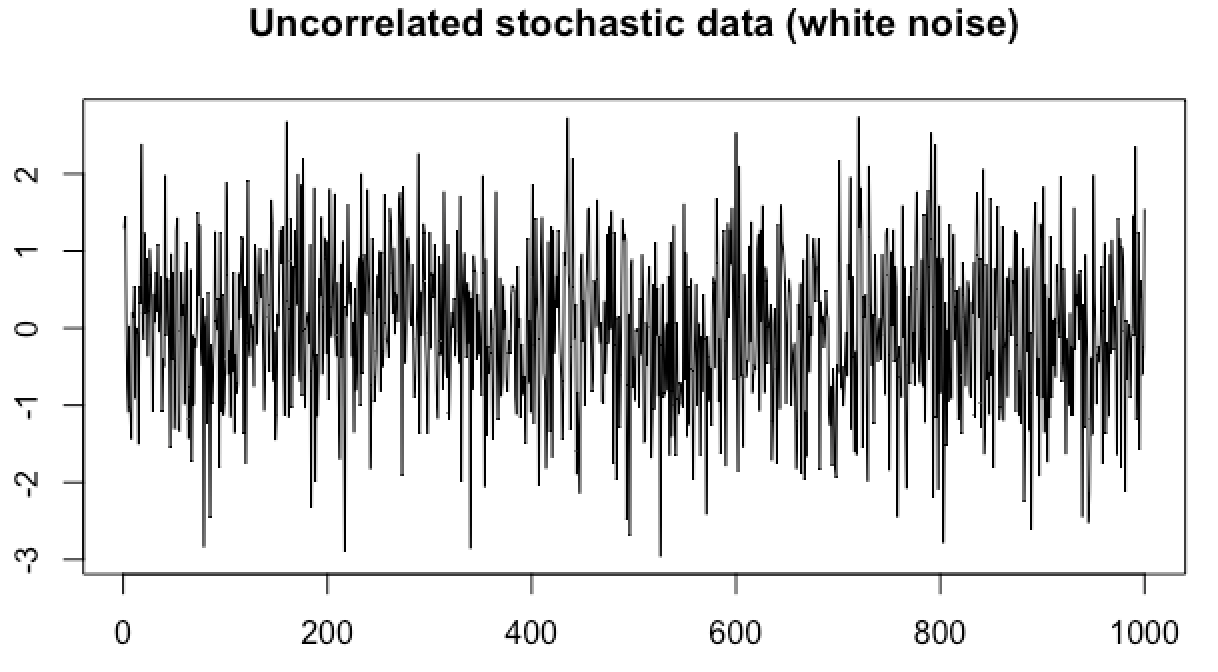
\includegraphics[width=0.25\linewidth]{figures/white_noise.png}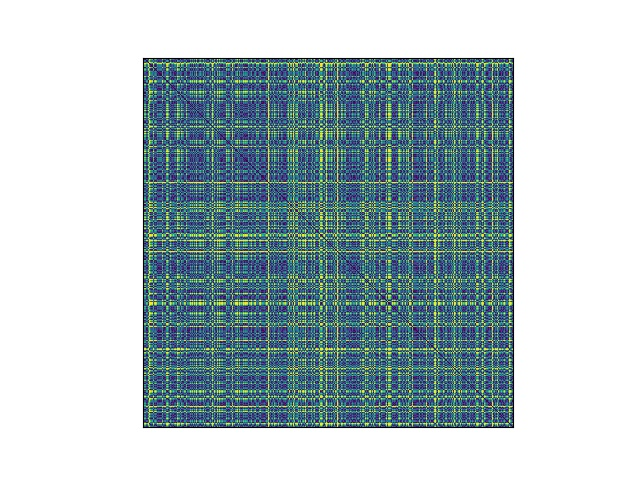
\includegraphics[width=0.25\linewidth]{figures/white_noise_R.jpg}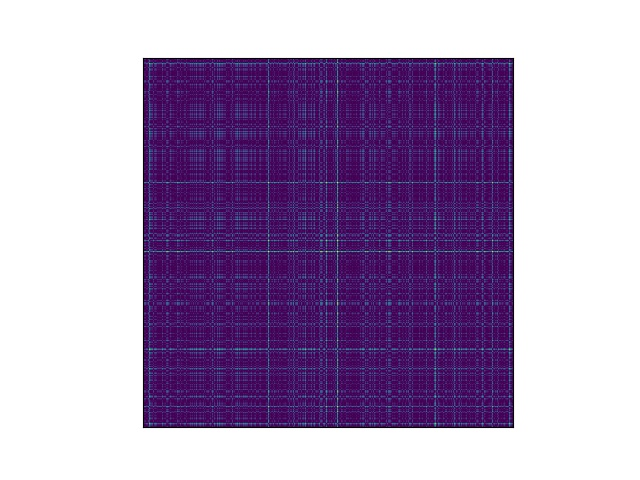
\includegraphics[width=0.25\linewidth]{figures/white_noise_GAF.jpg}\\
    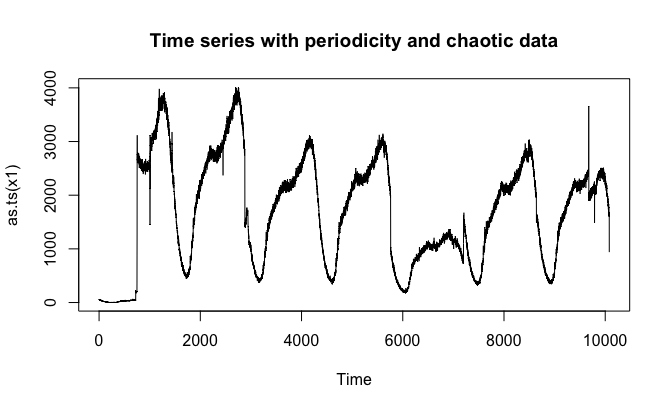
\includegraphics[width=0.25\linewidth]{figures/time_seires_with_frequency.png}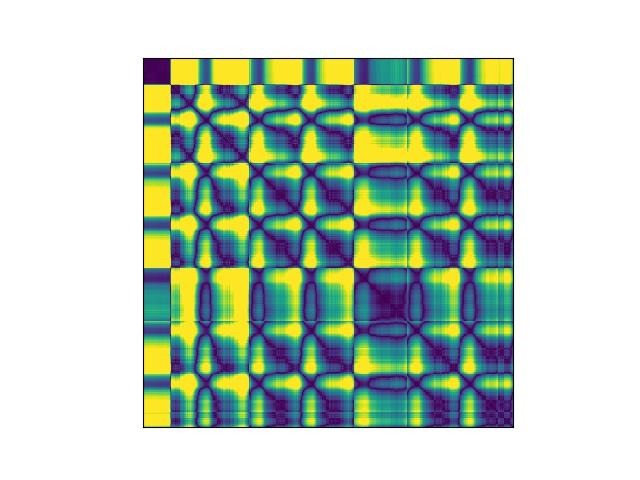
\includegraphics[width=0.25\linewidth]{figures/period_RP.jpg}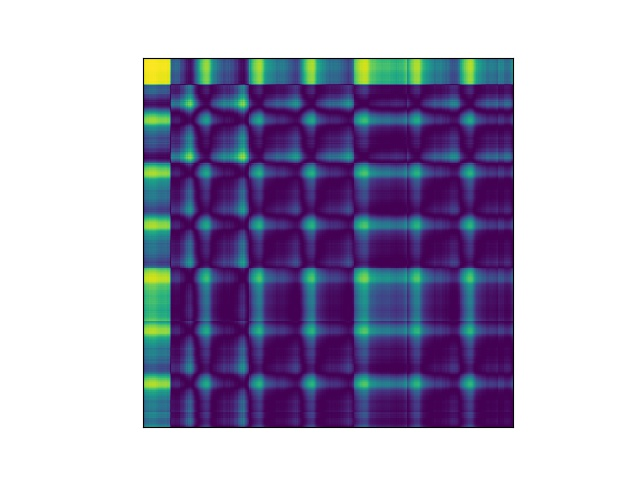
\includegraphics[width=0.25\linewidth]{figures/period_GAF.jpg}\\
    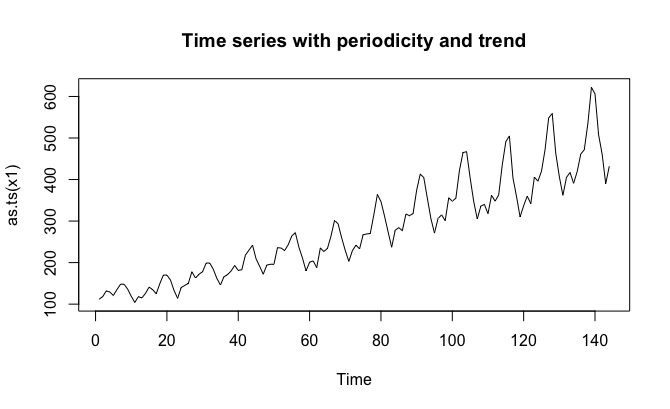
\includegraphics[width=0.25\linewidth]{figures/Period_data_with_linear_trend.png}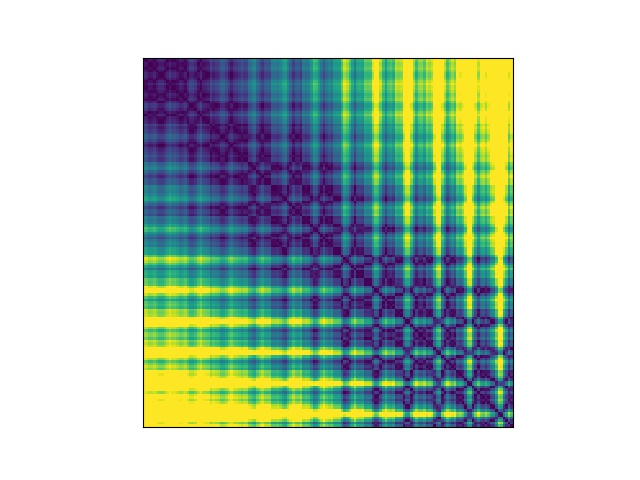
\includegraphics[width=0.25\linewidth]{figures/trend_period_RP.jpg}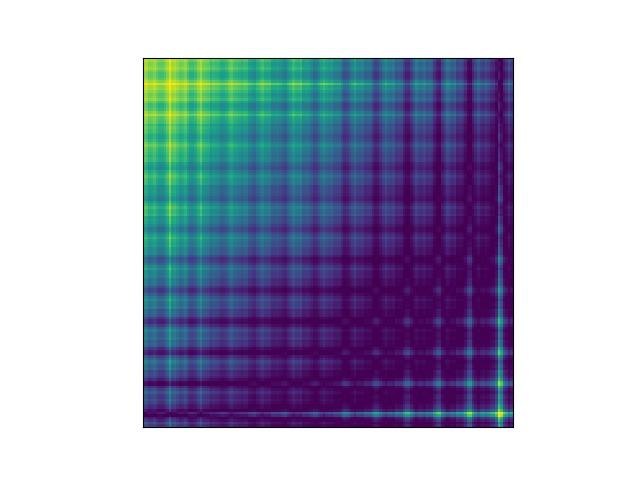
\includegraphics[width=0.25\linewidth]{figures/trend_period_GAF.jpg}\\
    \caption{Typical examples of recurrence plot(the second column) and Gramian Angular
      Field(the third column)}
  \label{fig:RP-egs}
\end{figure}

\end{frame}

\begin{frame}
  \frametitle{Image features}
  \begin{itemize}
  \item The original Bag of Features (BoF) model, which extracts features from one-dimensional
signal segments, has achieved a great success in time series classification
\citep{baydogan2013bag, wang2013bag}.
\item \citet{hatami2017bag} transform time-series into
two-dimensional recurrence images with recurrence plot \citep{eckmann1987recurrence} and
then applies the BoF model.

\item \citep{Razavian2014CNN} use the features acquired by the convolutional neural
  network as the input of the classifier, which significantly improves the accuracy of
  image classification.
  \end{itemize}
\end{frame}

\section{Image-based time series feature extraction}


\begin{frame}
  \frametitle{Image-based time series feature extraction}
  \framesubtitle{Scale-invariant feature transform (SIFT)}

  \begin{itemize}
  \item The scale space of an image is defined as the original image is convoluted with a
    variable-scale 2-dimensional Gaussian function.
  \item Key points are then taken as maxima/minima of the difference of Gaussians that occur at multiple scales.

  \item In our study, we use a 128-elements vector to characterize the key descriptors.
  \item Firstly, we establish an 8-direction histogram in each $4 \times 4$ sub-region, and a
    total of 16 sub-regions in the $16 \times 16$ region around the key point are
    calculated. Then we calculate the magnitude and direction of each pixel's gradient
    magnitude and add to the sub-region.
  \item In the end, a total of 128-dimensional image data based on histograms are
    generated.
  \item The sift method calculates the distribution characteristics of feature points in
    the whole image, and then generates a global histogram, so the spatial distribution
    information of the image is lost, and the image may not be accurately identified.

  \item A spatial pyramid method statistically distributes image feature points at
    different resolutions to obtain spatial information of images.
  \end{itemize}
\end{frame}

\begin{frame}
  \frametitle{Image-based time series feature extraction}
  \framesubtitle{Scale-invariant feature transform (SIFT)}

\begin{figure}
  \centering 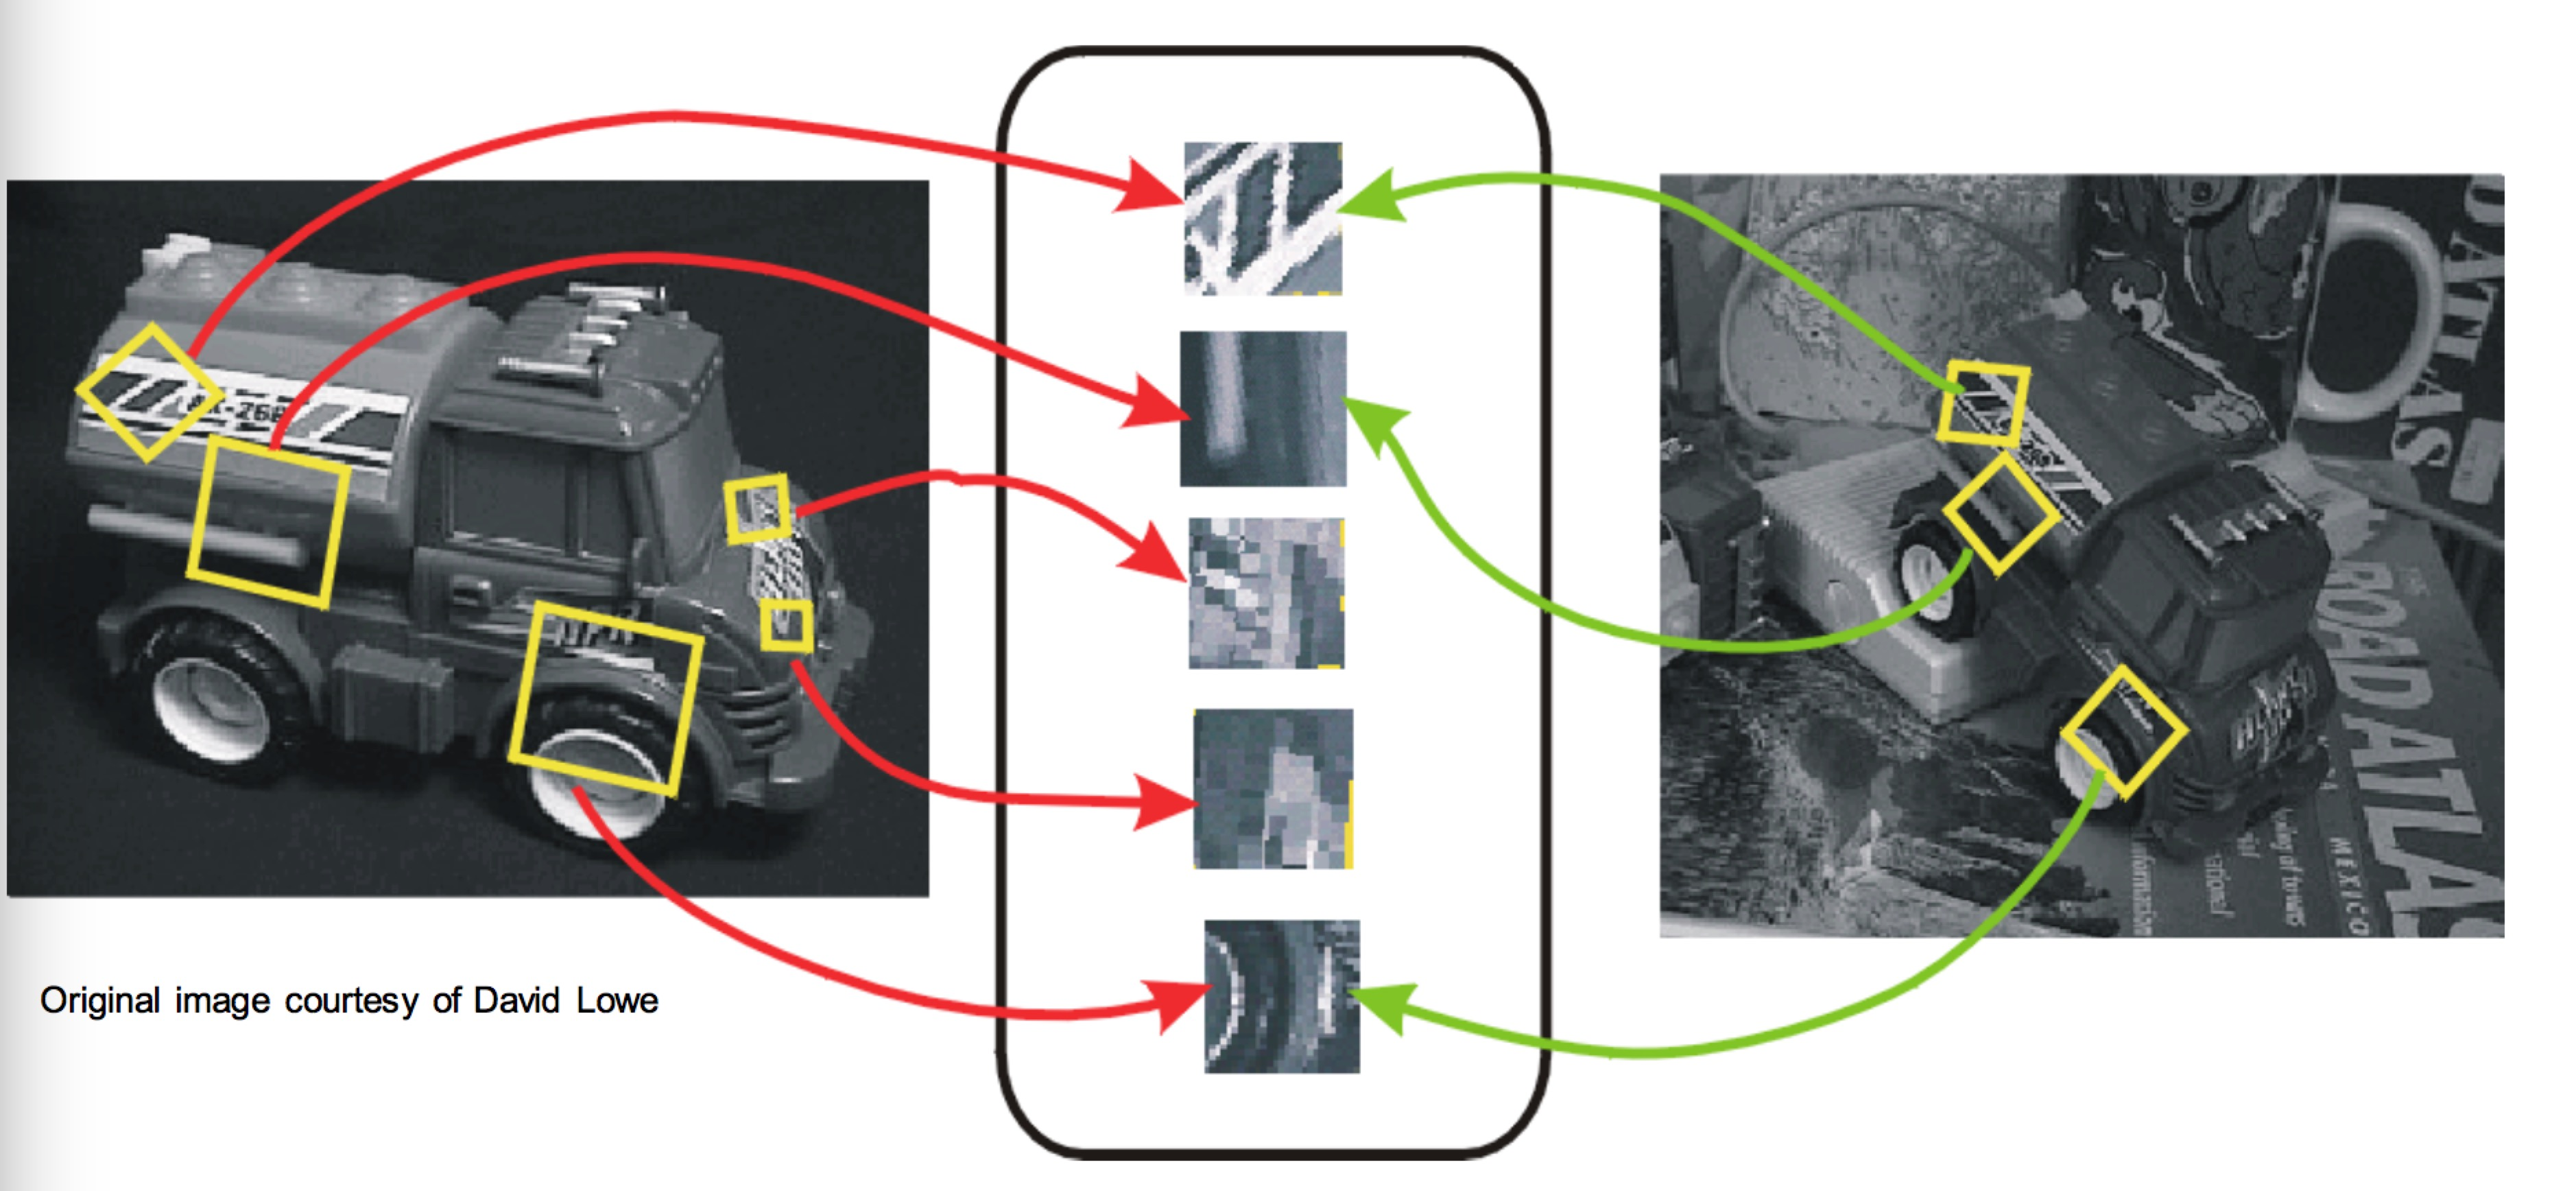
\includegraphics[width=1\linewidth]{figures/sift.png}
  \caption{Image feature extraction with scale-invariant feature transform}
  \label{fig:Feature extraction with SIFT}
\end{figure}

\end{frame}


\begin{frame}
  \frametitle{Image-based time series feature extraction}
  \framesubtitle{Scale-invariant feature transform (SIFT)}

\begin{figure}
  \centering 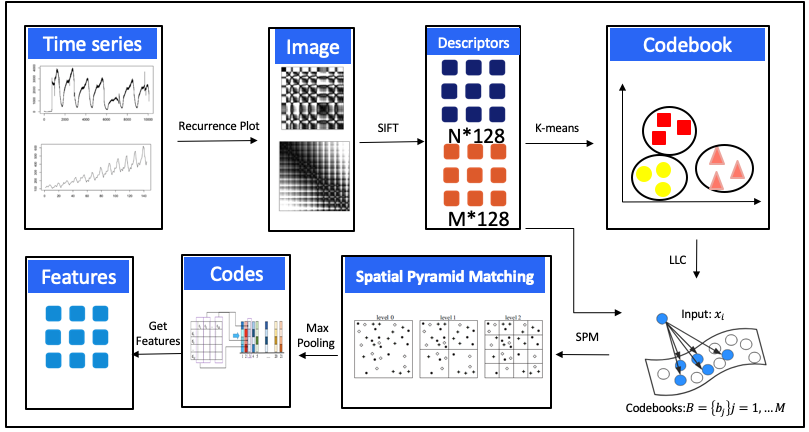
\includegraphics[width=1\linewidth]{figures/feature_extraction_sift.png}
  \caption{Image feature extraction with scale-invariant feature transform}
  \label{fig:Feature extraction with traditional image processing method}
\end{figure}

\end{frame}

\begin{frame}[allowframebreaks]
  \frametitle{Image-based time series feature extraction}
  \framesubtitle{Transfer learning with fine-tuning}

  \begin{itemize}
  \item The deep convolutional neural networks has greater advantages in accuracy compared
    with the traditional image features.

  \item But building models from scratch is complex and time consuming.

  \item One could used a pretrained trained neural network model and make adjustments to
    her own task -- \textbf{Transfer learning}.

  \item The pretrained model is based on \textbf{ImageNet} competition \citep{Deng2009ImageNet}.
    \begin{figure}
      \centering
      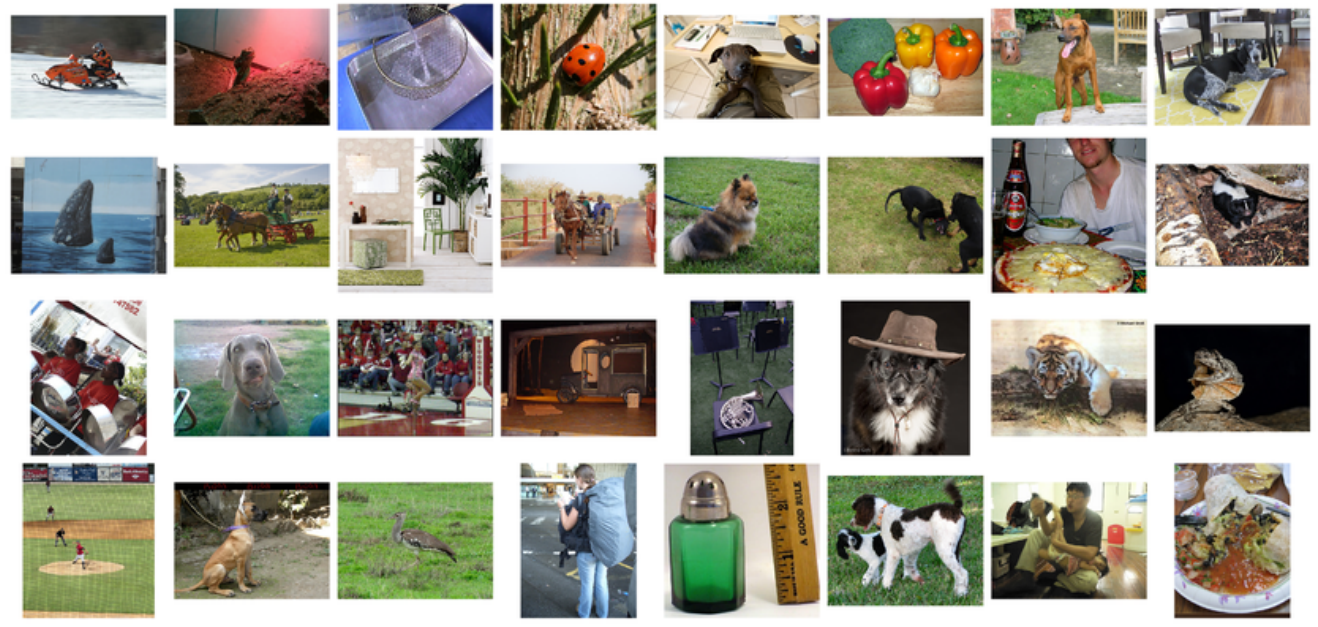
\includegraphics[width=0.9\linewidth]{figures/Sample-ImagesNet}
    \end{figure}

  \item The deep neural network models used for transfer learning

    \begin{itemize}
    \item ResNet\citep{Szegedy2016Inception}, Deep Residual Learning for Image Recognition
    \item Inception\citep{Szegedy2016Rethinking}, Evolved From GoogLeNet, merged with ResNet idea for image classification
    \item VGG\citep{Simonyan2014Very}, Very Deep Convolutional Networks for Large-Scale Image Recognition
    \end{itemize}


  \item With the pre trained model, we fix the parameters of the previous layers, and
    fine-tune the next few layers for our task. In this way, the speed of network training
    will be greatly accelerated.

  \end{itemize}
\end{frame}


\begin{frame}
  \frametitle{Image-based time series feature extraction}
  \framesubtitle{Transfer learning with fine-tuning}

\begin{figure}[thb]
  \centering
  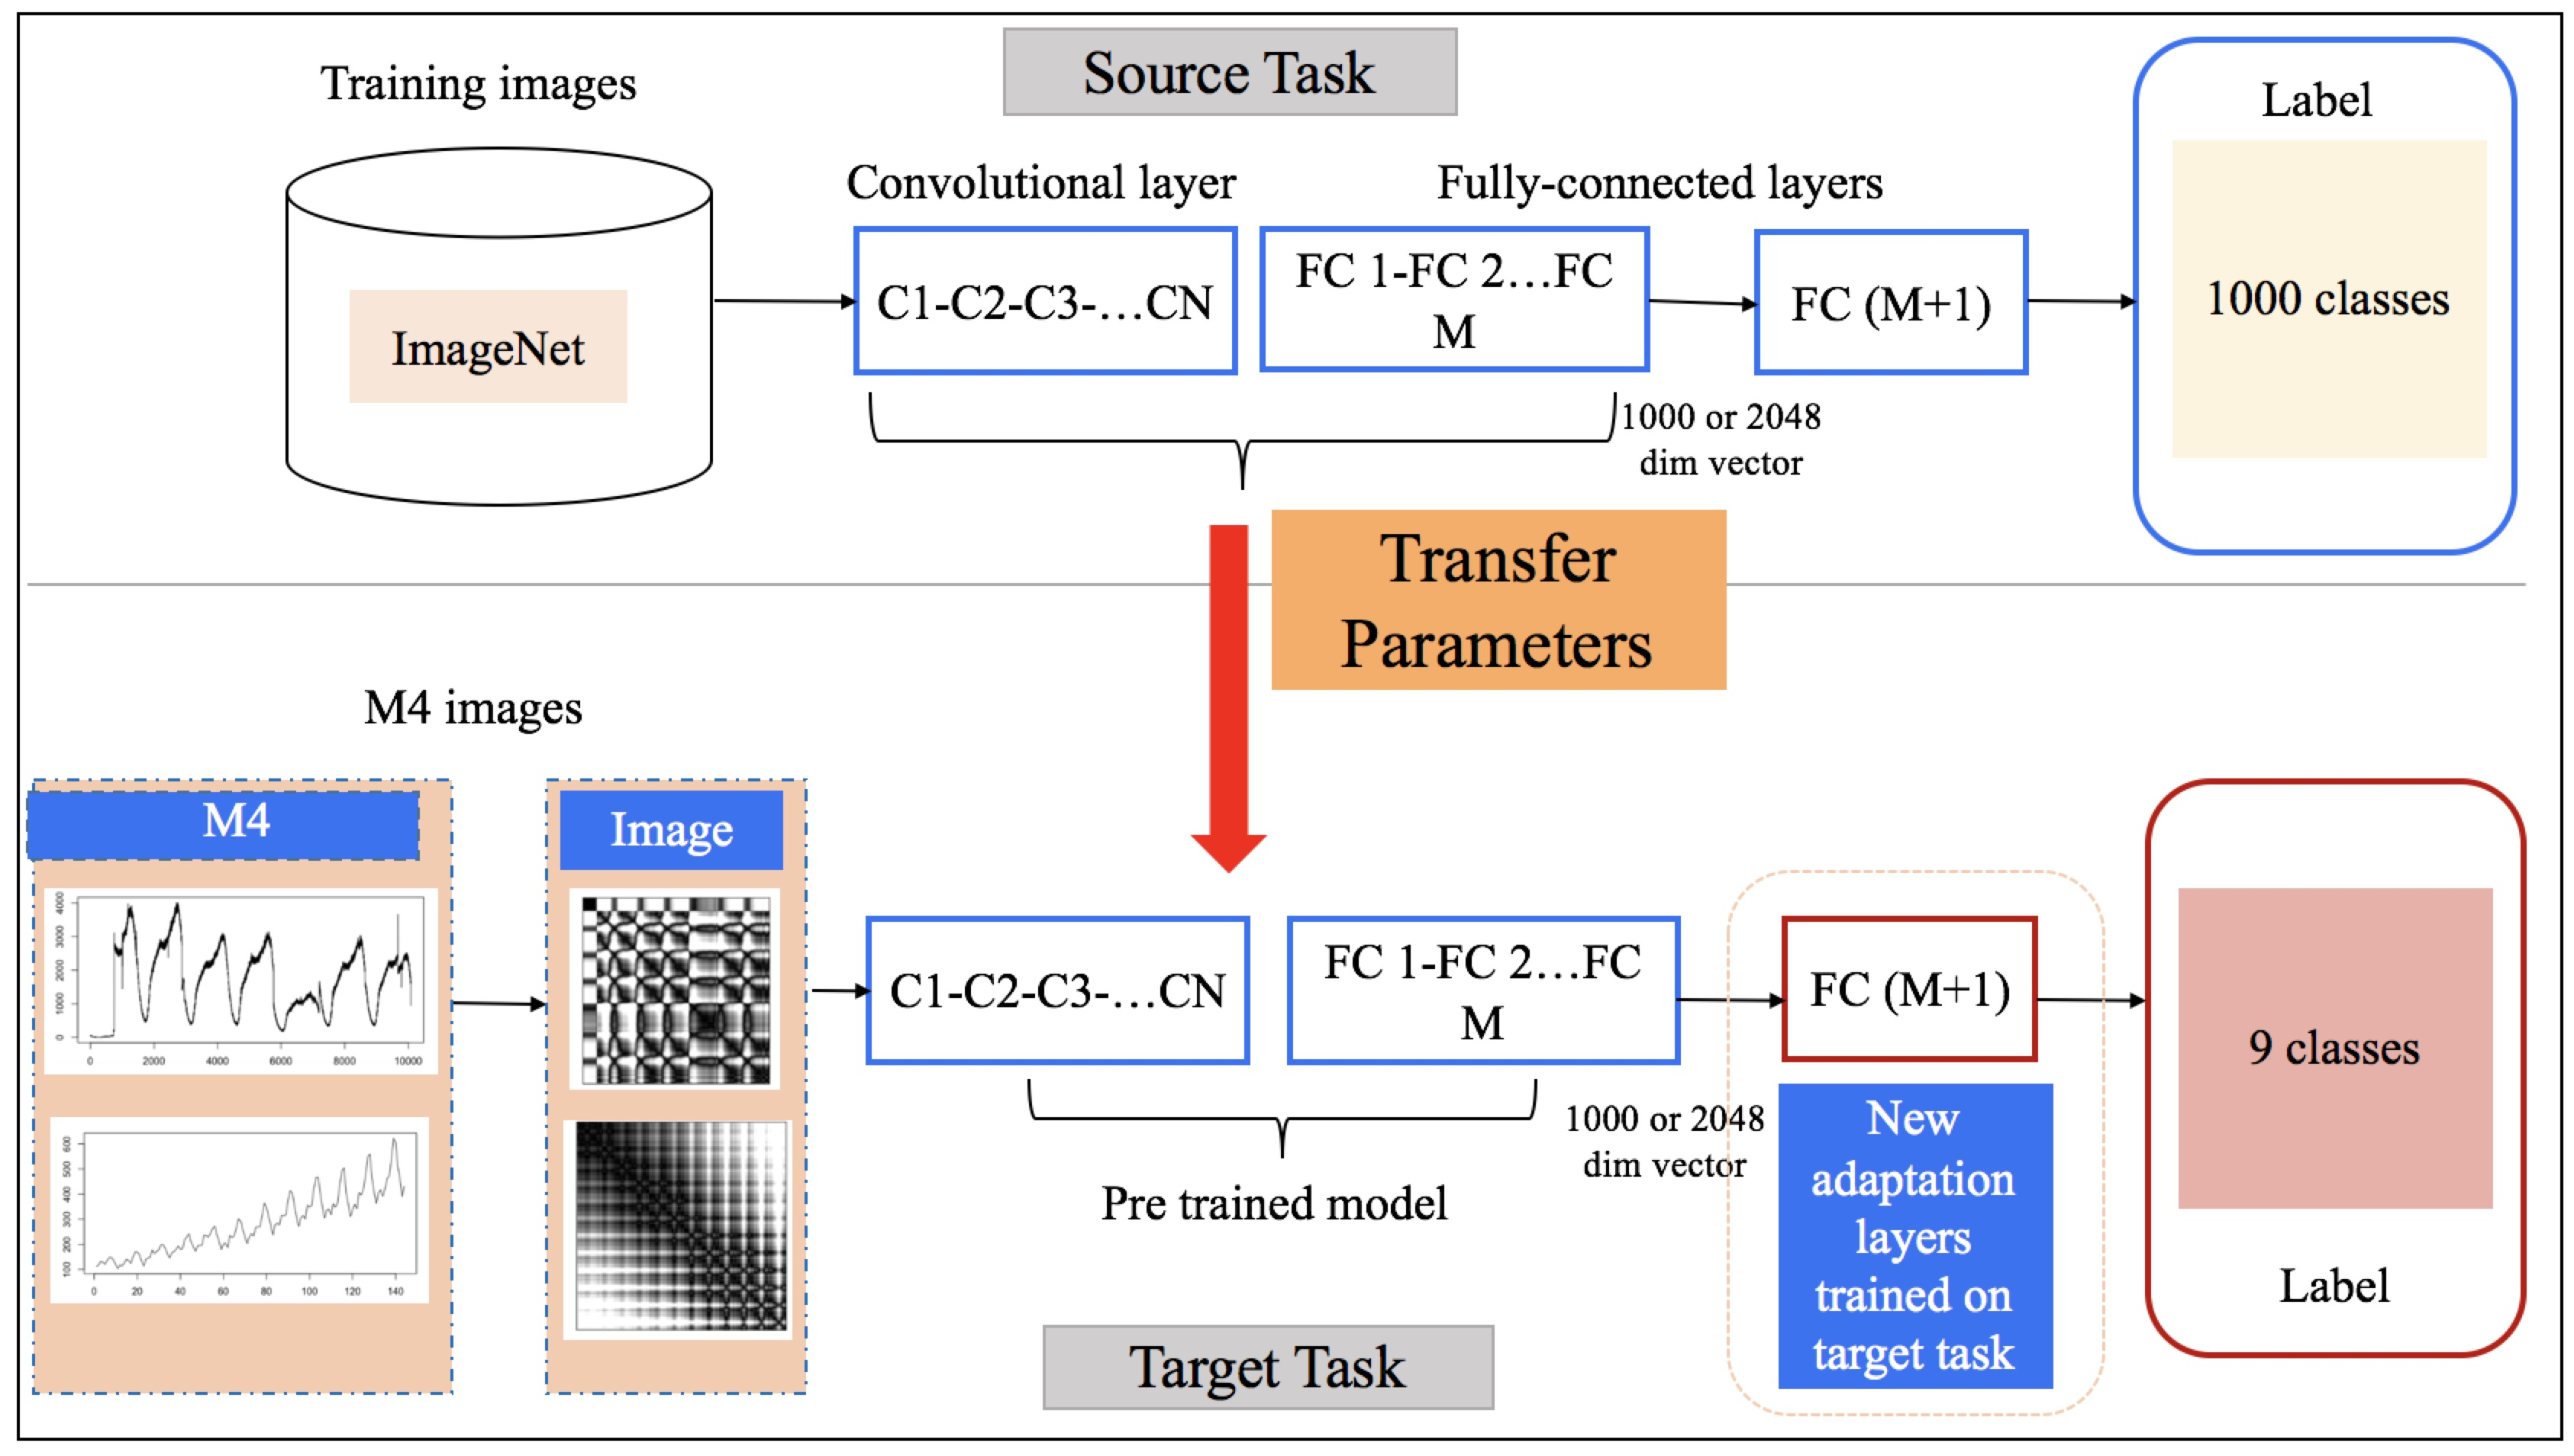
\includegraphics[width=0.8\linewidth]{figures/transfer-learning.jpg}
  \caption{\footnotesize{Transfer Learning-Fine-Tuning. }}
  \label{fig:transfer-learning}
\end{figure}
\end{frame}

\begin{frame}
  \frametitle{Time series forecasting methods}

  \begin{itemize}
\item \textbf{Naive}: uses the most recent observation as the forecast for all future periods.

\item \textbf{Seasonal naive}: forecasts are equal to the most recent observation from the
  corresponding time of year.

\item \textbf{The Theta method}: It performed particularly well in the M3-Competition proposed by
  \citet{Assimakopoulos2000The}.

\item \textbf{ETS}: exponential smoothing state space modeling, which is used widely as a general
  forecasting algorithm for trended and seasonal time series proposed by
  \citet{Hyndman2017A}.

\item \textbf{ARIMA}: autoregressive integrated moving average models, as implemented in the
  automated algorithm by \citet{HK08}.

\item \textbf{STL-AR}: an AR model is fitted to the seasonally adjusted series obtained from a STL
  decomposition proposed by \citet{cleveland1990stl}.

\item \textbf{Nnetar}: It fits a neural network model to a time series with lagged values of the
  time series as inputs (and possibly some other exogenous inputs).

\item \textbf{Rw-drift}: Random Walk with Drift.

\item \textbf{Tbats}: A Tbats model differs from dynamic harmonic regression in that the
  seasonality is allowed to change slowly over time in a Tbats model, while harmonic
  regression terms force the seasonal patterns to repeat periodically without changing, as
  implemented in the automated algorithm by \citet{HK08}.
\end{itemize}
\end{frame}

\section{Forecast-model averaging}


\begin{frame}
  \frametitle{Forecast loss measurement}
  \begin{itemize}
  \item \textbf{Forecast loss measurement}: Overall Weighted Average (OWA) is an indicator
    of two accuracy measures: the Mean Absolute Scaled Error (MASE) and the symmetric Mean
    Absolute Percentage (sMAPE).

\begin{equation*}
  \begin{aligned}
    \mathrm{sMAPE}&=\frac{1}{h}\sum_{t=1}^h\frac{2\mid Y_{t}-\widehat{Y_{t}}\mid}{\mid Y_{t}\mid+\mid\widehat{Y_{t}} \mid},\\
    \mathrm{MASE}&=\frac{1}{h}\frac{\sum_{t=1}^h\mid Y_{t}-\widehat{Y_{t}} \mid}{\frac{1}{n-m}\sum_{t=m+1}^n\mid Y_{t}-Y_{t-m} \mid},\\
    \mathrm{OWA}&=\frac{\mathrm{sMAPE /sMPAE + MASE/MASE}}{2},
  \end{aligned}
\end{equation*}



\item Train a high dimensional regression model (Lasso) with $X_{train}$ and $M ASE$
\item Calculate predicted $MASE$ with $X_{test}$.
\end{itemize}

\end{frame}

\begin{frame} {Forecast-model averaging}
  \begin{figure}%[!thb]
  \centering
  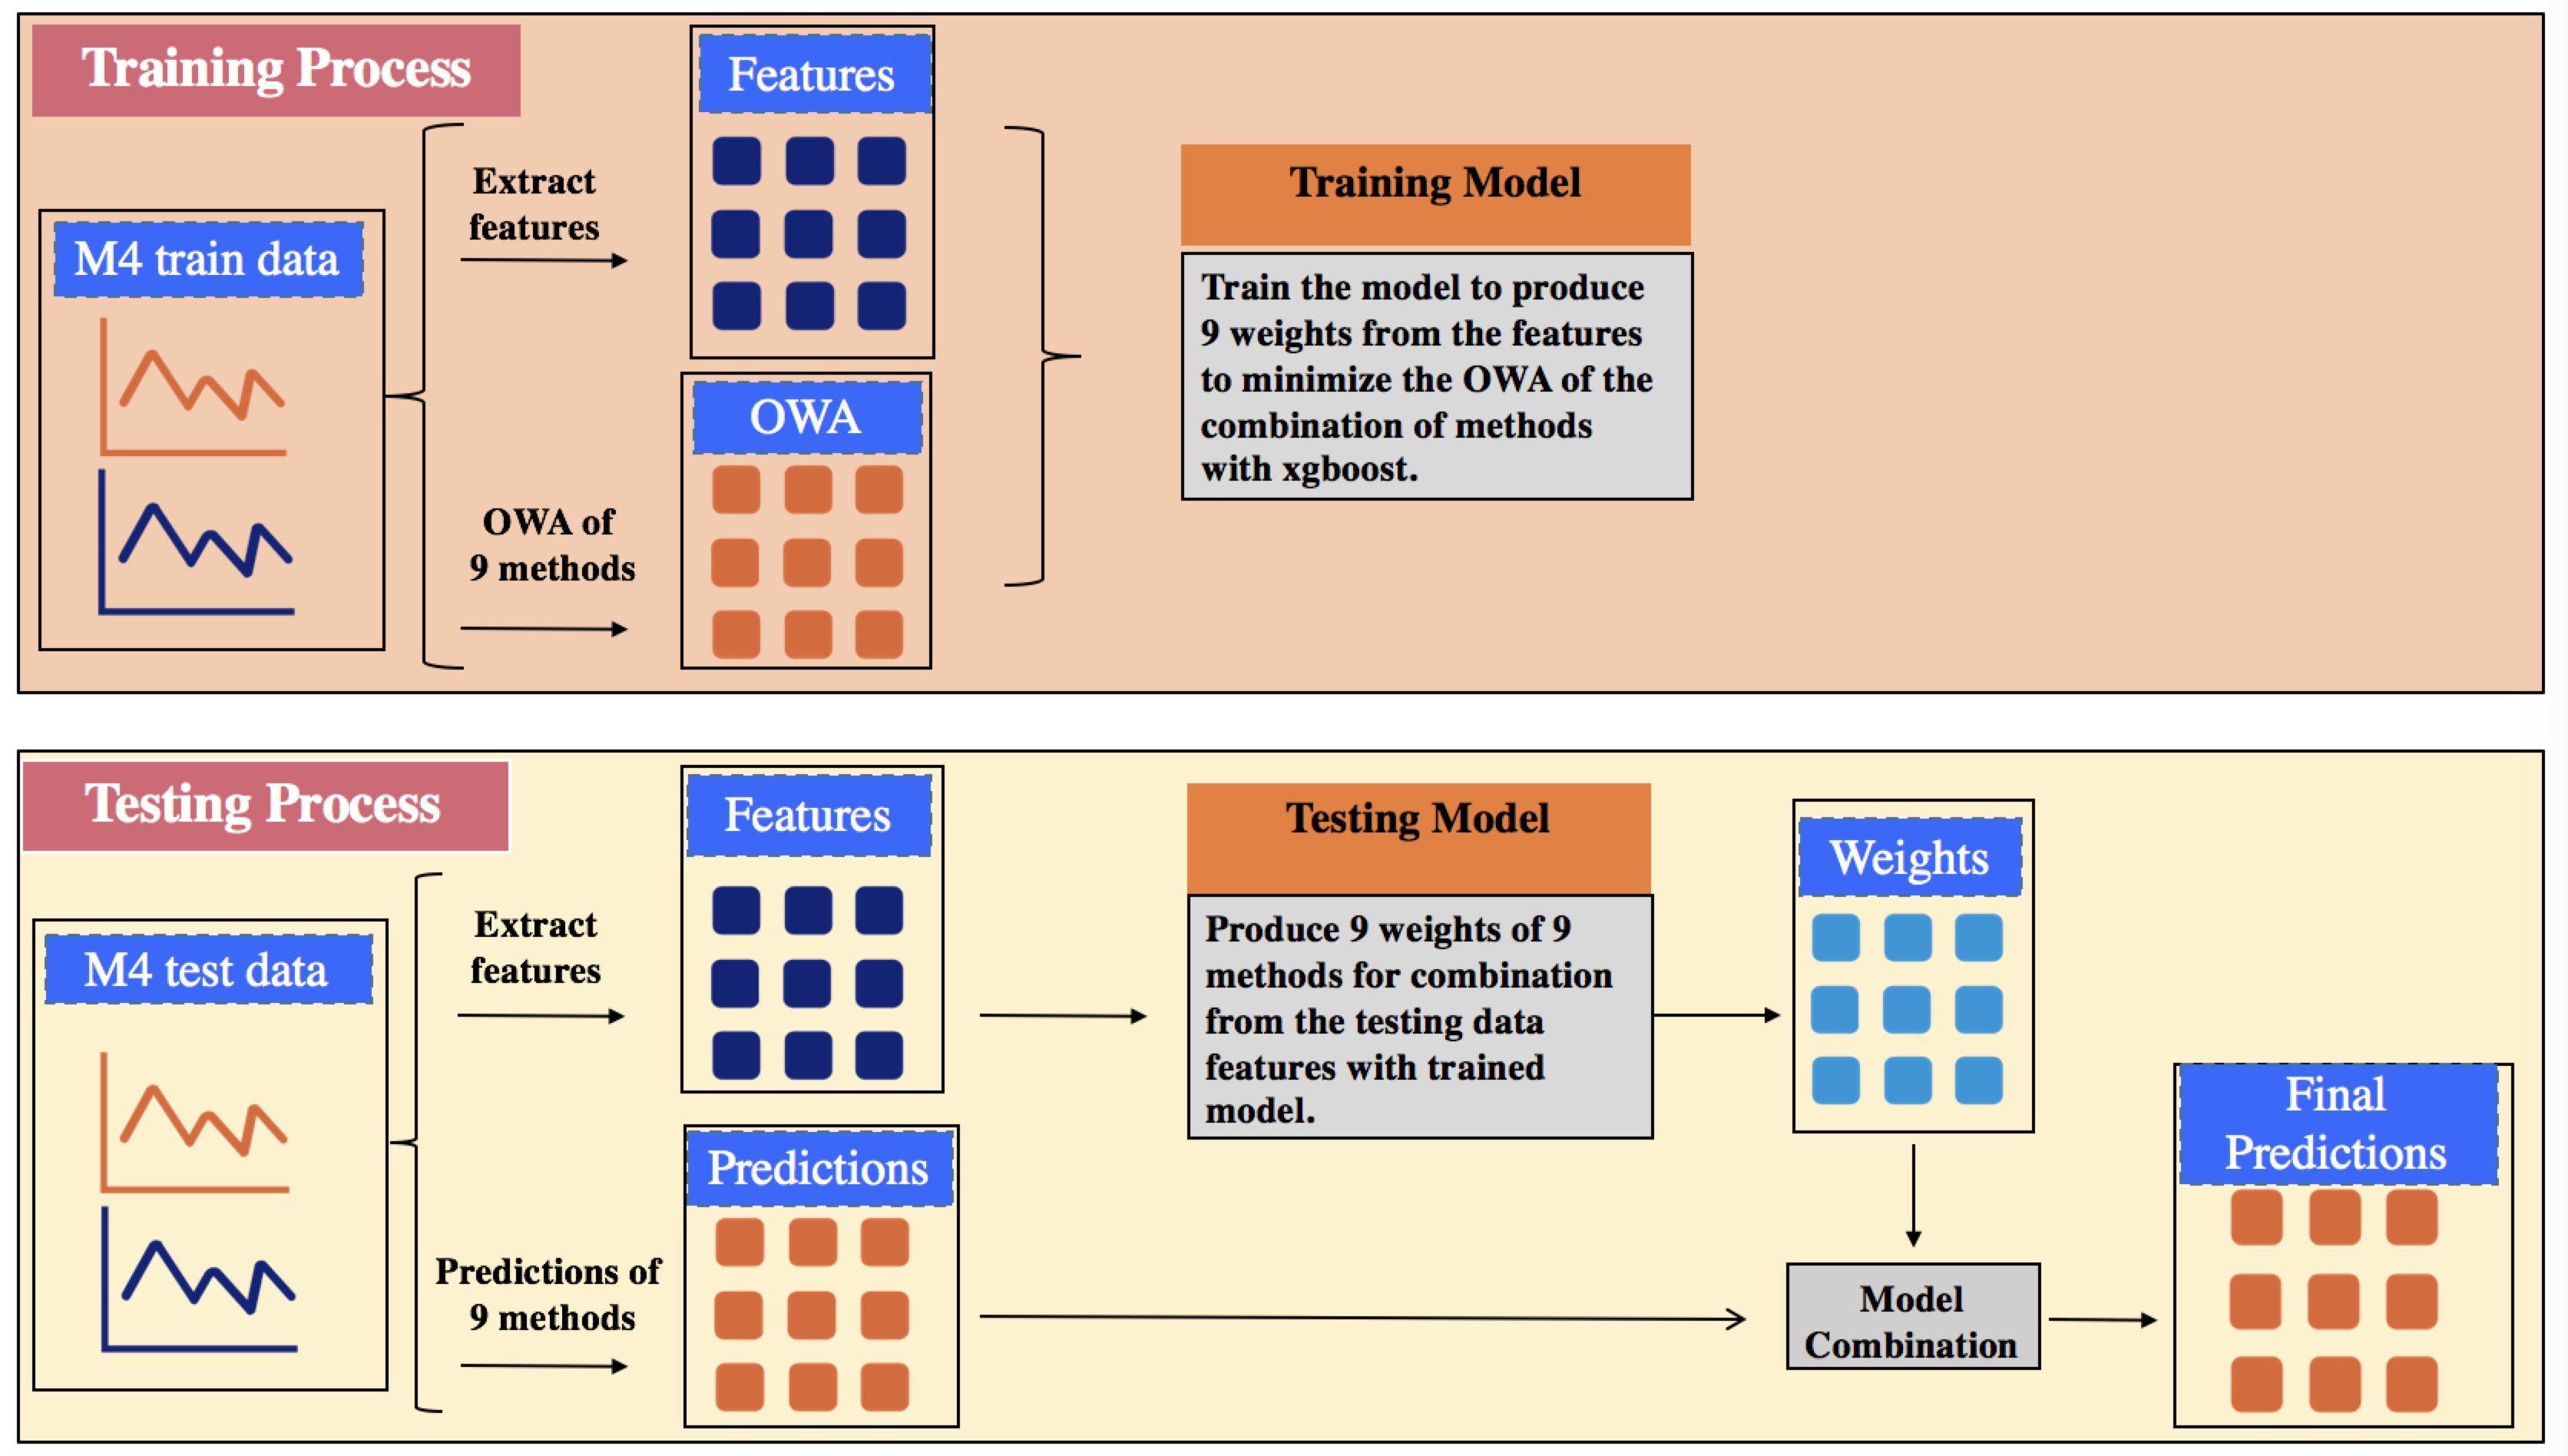
\includegraphics[width=1\linewidth]{figures/model_averaging1.png}
  % \caption{Framework of forecast model averaging for the largest time series forecasting
  %   competition dataset M4 based on automatic feature extraction.}
  \label{fig:framework}
\end{figure}

\end{frame}


\begin{frame}
  \frametitle{Forecast-model averaging}
  \begin{itemize}

\item In order to get the weight $w(f_{n})_{m}$ for every method, softmax transform is carried on the output $p(f_{n})_{m}$  .
\begin{equation*}
  \begin{aligned}
   w(f_{n})_{m}=\frac{e^{p(f_{n})_{m}}}{\sum_{m}e^{p(f_{n})_{m}}}
  \end{aligned}
\end{equation*}

\item The weighted average loss function is minimized:

  \begin{equation*}
  \begin{aligned}
    \mathrm{argmin}_{w}\overline { L }_ { n }  =\sum\nolimits_{m=1}^{M}w(f_{n})_{m}O_{nm}
  \end{aligned}
\end{equation*}
\end{itemize}

% \begin{figure}[htb]
%   \centering
  % 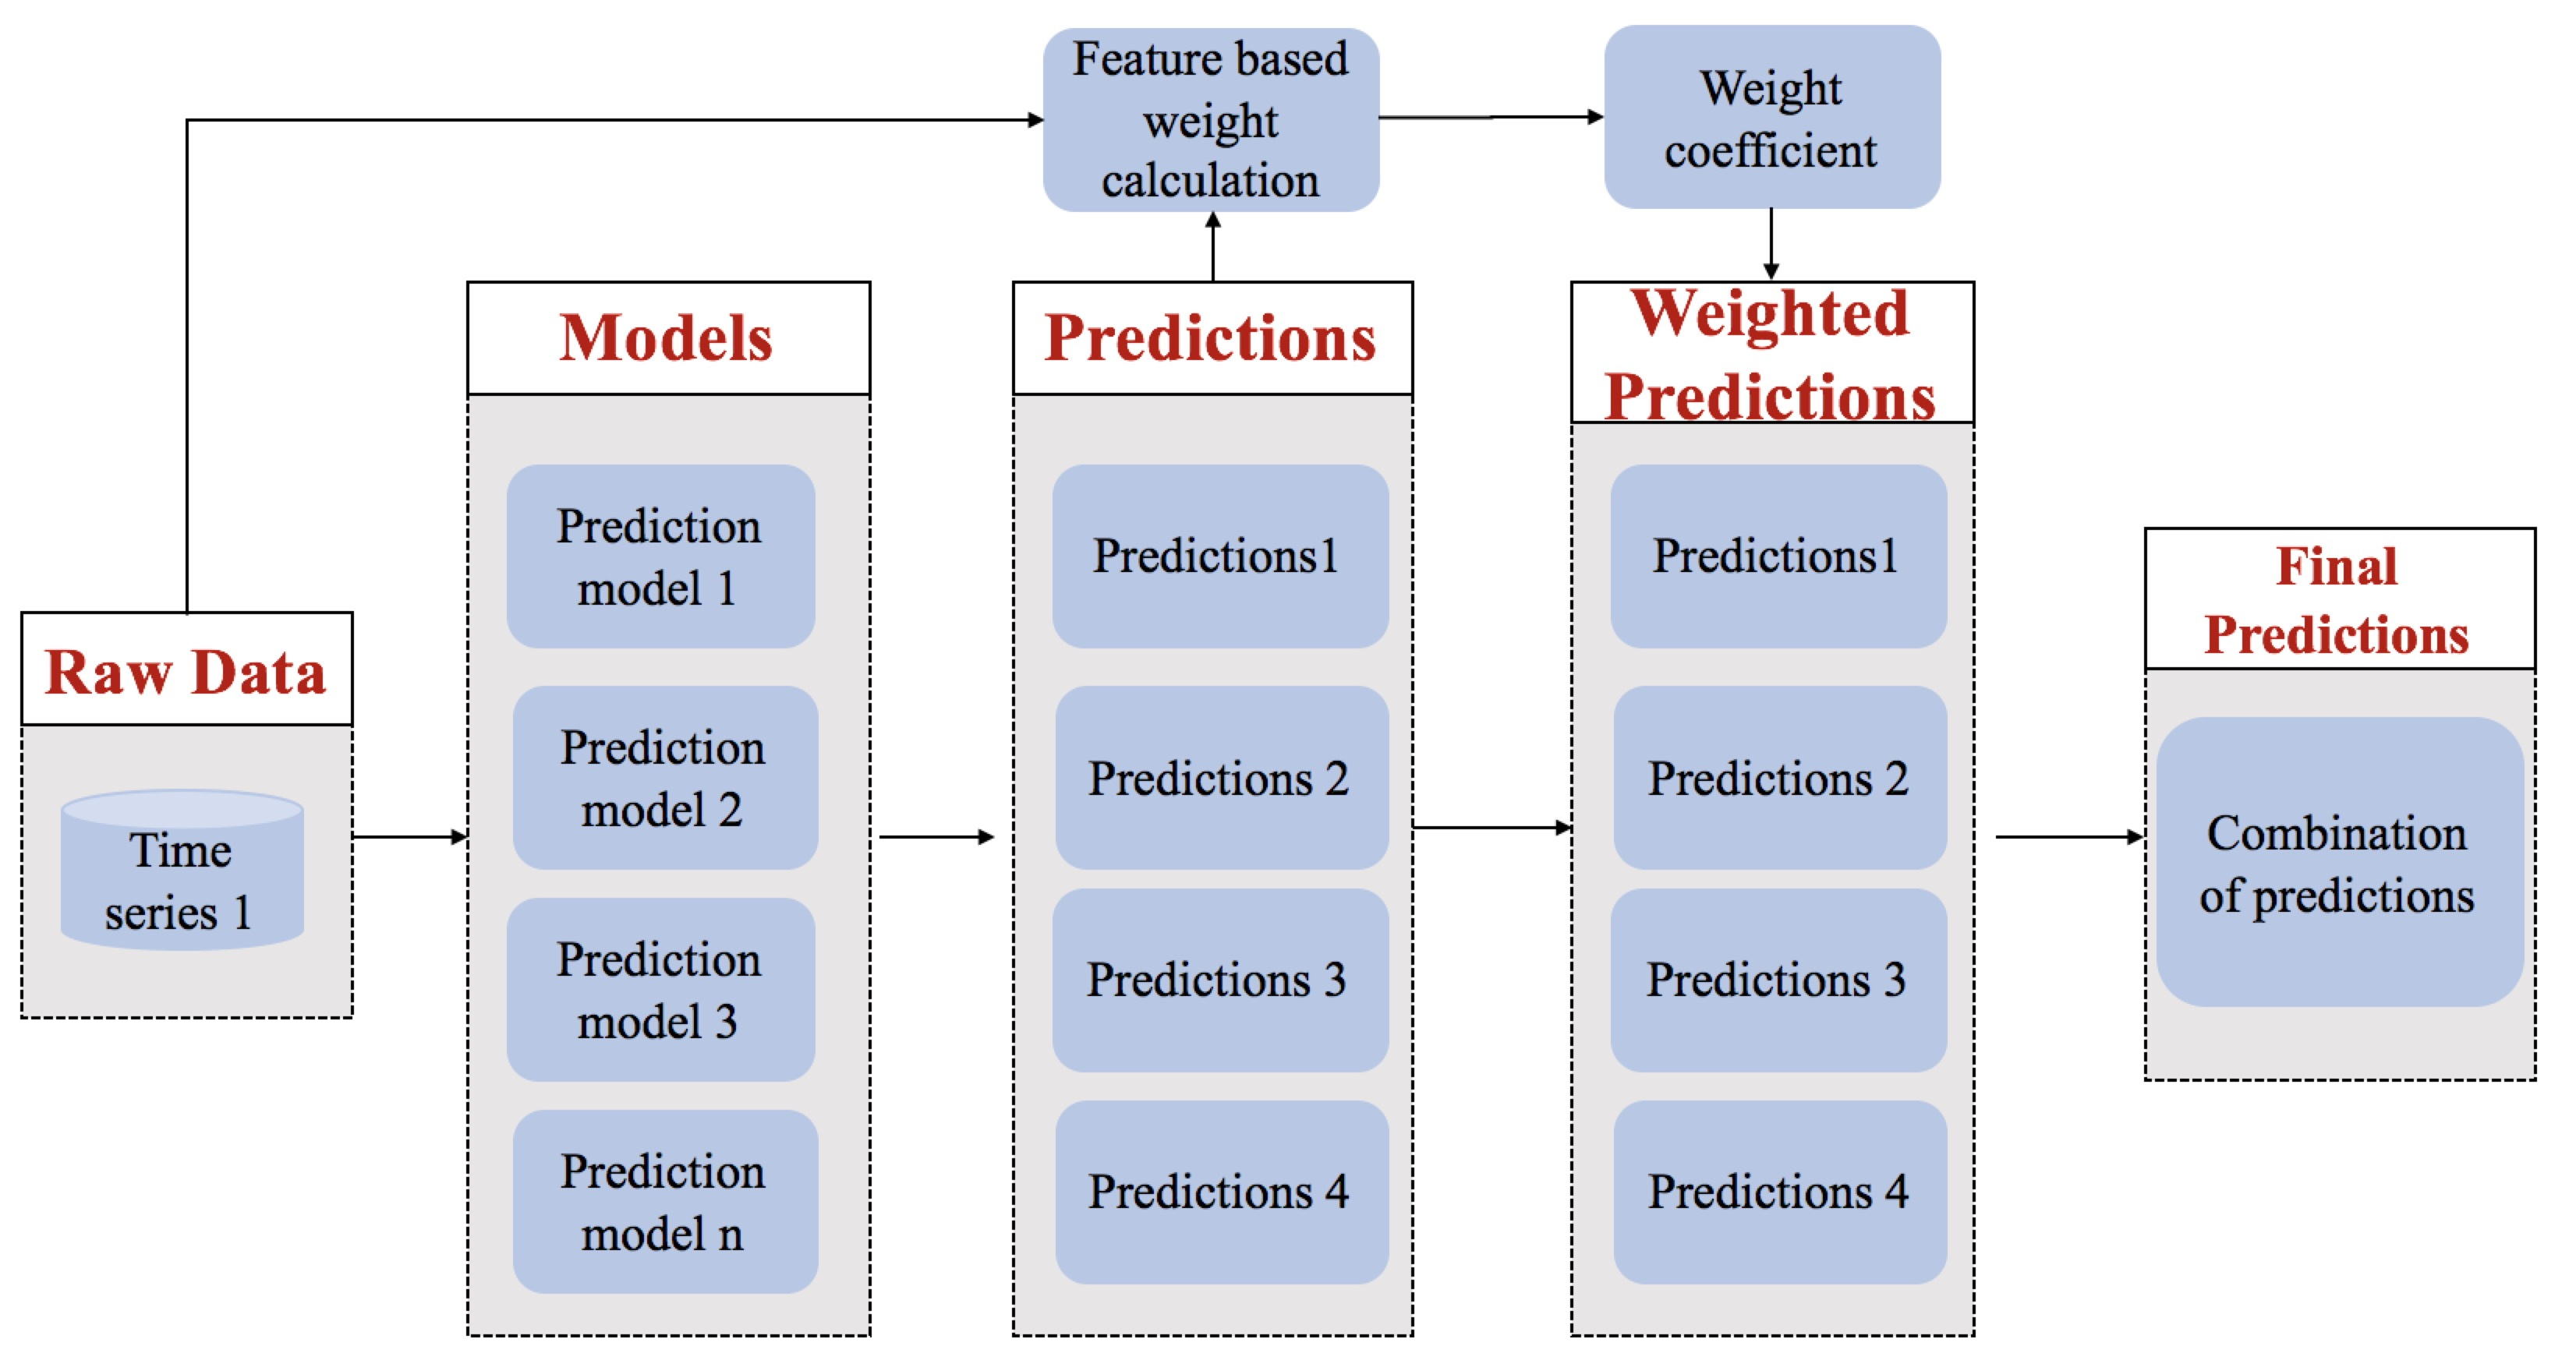
\includegraphics[width=0.7\linewidth]{figures/model-averging-feature-based}
  % \caption{Model averaging framework based on automatic feature extraction for the largest
  %   time series forecasting competition dataset.}
%   \label{fig:framework}
% \end{figure}

\end{frame}


\begin{frame}
  \frametitle{Forecast-model averaging}


\begin{table}
  \centering
  \caption{Forecast-model averaging compared with M4 competition in sMAPE.}
  \label{sMAPE_MA}
  \resizebox{\linewidth}{!}{
    \begin{tabular}{llllllll}
      \toprule
      Rank        & Yearly & Quarterly & Monthly & Weekly & Daily & Hourly & Total \\
      \midrule
      \multicolumn{8}{c}{M4 competition}   \\
      1 & 13.176 & 9.679 & 12.126 & 7.817 & 3.170 & 9.328 & 11.374 \\
      2 & 13.528 & 9.733 & 12.639 & 7.625 & 3.097 & 11.506 & \textbf{11.720} \\
      3 & 13.943 & 9.796 & 12.747 & 6.919 & 2.452 & 9.611 & 11.845 \\
      4 & 13.712 & 9.809 & 12.487 & 6.814 & 3.037 & 9.934 & 11.695 \\
      5 & 13.673 & 9.816 & 12.737 & 8.627 & 2.985 & 15.563 & 11.836 \\
      6 & 13.669 & 9.800 & 12.888 & 6.726 & 2.995 & 13.167 & 11.897 \\
      7 & 13.679 & 10.378 & 12.839 & 7.818 & 3.222 & 13.466 & 12.020 \\
      8 & 13.366 & 10.155 & 13.002 & 9.148 & 3.041 & 17.567 & 11.986 \\
      9 & 13.910 & 10.000 & 12.780 & 6.728 & 3.053 & 8.913 & 11.924 \\
      10 & 13.821 & 10.093 & 13.151 & 8.989 & 3.026 & 9.765 & 12.114 \\
      \midrule
      % $SIFT+XGBoost(9 methods)$ & 13.935 & 9.855 & 12.656 & 8.502 & 3.175 & 11.913 & 11.859\\
      % $SIFT+XGBoost(8 methods)$ & 13.896 & 9.863 &  \textbf{12.596} & 7.899 &  \textbf{3.063} & 11.772 & 11.816 \\
      $\textbf{SIFT}$ & 13.896 & 9.863 &  12.596 & 7.899 & 3.063 & 11.772 & \textbf{11.816} \\
      % $SIFT+XGBoost(5 methods)$ & 13.881 & 9.858 &  \textbf{12.625} & 8.289 &  \textbf{3.017} & 12.296 & 11.824 \\
      $\textbf{CNN}$\\
      $inception-v1+XGBoost$ & 13.862 & 9.835 & 12.616 & 8.255 & 3.117 & 12.173 & 11.815\\
      $resnet-v1-101+XGBoost$ &13.890  &9.810 &12.566  & 8.341  & 3.107 &11.772 &11.790     \\
      $resnet-v1-50+XGBoost$ &13.847  &9.840 & 12.549  & 8.033  & 3.113 &11.762 &\textbf{11.778}     \\
      $vgg-19+XGBoost$ &13.987  &9.838 & 12.583 &8.408  &3.077 &11.856 &11.826     \\
      % \midrule
      % \multicolumn{8}{c}{Model averaging+Gramian angular field}\\
      % $\textbf{Pre trained CNN model+Classifier}$\\
      % $inception-v1+XGBoost$      &13.926   &9.859       &\textbf{12.639}  &8.161    &3.103  &12.077  &11.846  \\
      % $resnet-v1-101+XGBoost$        &13.861   &9.811       &\textbf{12.597}  &7.851   &3.124   &11.933 &11.798   \\
      % $resnet-v1-50+XGBoost$       &13.914   &9.808       &\textbf{12.574}  &7.887    &\textbf{3.067}   &11.882  &11.796    \\
      % $vgg-19+XGBoost$       &13.949    &9.868       &\textbf{12.617}   &7.937   &\textbf{3.070}   &12.078    &11.839   \\

      \bottomrule
    \end{tabular}
  }
\end{table}
\end{frame}




\begin{frame}
  \frametitle{Forecast-model averaging}

\begin{table}
  \centering
  \caption{Forecast-model averaging compared with  M4 competition in OWA.}
  \label{owa_MA}
  \resizebox{\linewidth}{!}{
    \begin{tabular}{llllllll}
      \toprule
      Rank        & Yearly & Quarterly & Monthly & Weekly & Daily & Hourly & Total \\
      \midrule
      \multicolumn{8}{c}{M4 competition}\\
      1 & 0.778 & 0.847 & 0.836 & 0.851 & 1.046 & 0.440 & 0.821 \\
      2 & 0.799 & 0.847 & 0.858 & 0.796 & 1.019 & 0.484 & \textbf{0.838} \\
      3 & 0.820 & 0.855 & 0.867 & 0.766 & 0.806 & 0.444 & 0.841 \\
      4 & 0.813 & 0.859 & 0.854 & 0.795 & 0.996 & 0.474 & 0.842 \\
      5 & 0.802 & 0.855 & 0.868 & 0.897 & 0.977 & 0.674 & 0.843 \\
      6 & 0.806 & 0.853 & 0.876 & 0.751 & 0.984 & 0.663 & 0.848 \\
      7 & 0.801 & 0.908 & 0.882 & 0.957 & 1.060 & 0.653 & 0.860 \\
      8 & 0.788 & 0.898 & 0.905 & 0.968 & 0.996 & 1.012 & 0.861 \\
      9 & 0.836 & 0.878 & 0.881 & 0.782 & 1.002 & 0.410 & 0.865 \\
      10 & 0.824 & 0.883 & 0.899 & 0.939 & 0.990 & 0.485 & 0.869 \\
      \midrule
      % $SIFT+XGBoost(maxDepth=14)$ & 0.82 & 0.85 & 0.89 & 0.92 & 1.04 & 0.50 & 0.86 \\
      % $SIFT+XGBoost(9 methods)$ & 0.822 & 0.859 & 0.873 & 0.951 & 1.050 & 0.499 & 0.854 \\
      % $SIFT+XGBoost(8 methods)$ & 0.820 & 0.858 & 0.863 & 0.839 & \textbf{1.009} & 0.498 & 0.848 \\
      $\textbf{SIFT} $ & 0.820 & 0.858 & 0.863 & 0.839 & 1.009 & 0.498 & \textbf{0.848} \\
      % $SIFT+XGBoost(5 methods)$ & 0.818 & 0.855 & 0.874 & 0.878 & \textbf{0.985} & 0.522 & 0.849 \\
      $\textbf{CNN}$\\
      $inception-v1+XGBoost$ & 0.816 & 0.856 & 0.880 & 0.880 & 1.022 & 0.511 & 0.852 \\
      $resnet-v1-101+XGBoost$ &0.817  &0.855 &0.868  &0.880  &1.021 &0.497 &\textbf{0.848}     \\
      $resnet-v1-50+XGBoost$ &0.815  &0.856 &0.884  &0.866  &1.023 &0.498 &0.852     \\
      $vgg-19+XGBoost$ &0.825  &0.857 &0.878  &0.878  &1.011 &0.502 &0.854     \\
      % \midrule
      % \multicolumn{8}{c}{Model averaging+Gramian angular field}\\
      % $\textbf{Pre trained CNN model+Classifier}$\\
      % $inception-v1+XGBoost$    & 0.822 & 0.859 & 0.867 & 0.857 & 1.021 & 0.501 & 0.851      \\
      % $resnet-v1-101+XGBoost$      & 0.816 & 0.855 & 0.882 & 0.831 & 1.028 & 0.504 & 0.852   \\
      % $resnet-v1-50+XGBoost$          & 0.819 & 0.855 & 0.886 & 0.836 & \textbf{1.016} & 0.502 & 0.854\\
      % $vgg-19+XGBoost$        & 0.821 & 0.858 & 0.884 & 0.843 & \textbf{1.017} & 0.510 & 0.855 \\
      \bottomrule
    \end{tabular}
  }
\end{table}

\end{frame}


\begin{frame}
  \frametitle{Ongoing work}

  \begin{itemize}
  \item Python package: {\color{blue} \texttt{forecasttsimaging}} in preparation.
  \item Train the imaging forecasting model with {\color{blue} \texttt{GRATIS}} \citep*{kang2019gratis}.

  \item Related time series forecasting.
  \item Automatic selection of \emph{p}, \emph{d} and \emph{q} in ARIMA with time series imaging.

  \item The automatic extracted features are usually\textbf{ not interpretable}.  This
    allows for statistical forecasting when data privacy is a real concern.

  \end{itemize}

\end{frame}
\begin{frame}[plain]
  \addtocounter{framenumber}{-1}
  \begin{center}
    {\color{SUblue} \textbf{\Huge Thank you!}}
    \vspace{1cm}

    {\texttt{\textbf{\url{feng.li@cufe.edu.cn}}}}

    \vspace{1cm}

    {\texttt{\textbf{\url{http://feng.li/}}}}

  \end{center}
\end{frame}

\begin{frame}%[allowframebreaks]
  \frametitle{References}
  \tiny
\bibliography{tsforecast-image}
\bibliographystyle{agsm}
\end{frame}

\end{document}
